\documentclass[svgnames]{beamer}


\mode<presentation>
{
  \usetheme[titleformat=smallcaps,numbering=fraction,progressbar=frametitle]{metropolis}
  \usecolortheme[light,accent=orange]{solarized}
  %\usecolortheme[named=Goldenrod]{structure}
  % or ...

  \setbeamercovered{transparent}
  % or whatever (possibly just delete it)
}


% \usepackage{mathtext}
\usepackage[utf8]{inputenc}
\usepackage[english,russian]{babel}
\usepackage{cmap}
\hypersetup{unicode=true}
\graphicspath{{images/}{slides/images}}


\title[CMTA 05] % (optional, use only with long paper }
{Text classification}

\subtitle
{Computational Methods for Text Analysis} % (optional)

\author%[Author, Another] % (optional, use only with lots of authors)
{Кирилл Александрович Маслинский}
% - Use the \inst{?} command only if the authors have different
%   affiliation.

\institute%[Universities of Somewhere and Elsewhere] % (optional, but mostly needed)
{НИУ ВШЭ Санкт-Петербург}
% - Use the \inst command only if there are several affiliations.
% - Keep it simple, no one is interested in your street address.

\date%[Short Occasion] % (optional)
{04.11.2020 / 05}

\subject{natural language processing, text mining}
% This is only inserted into the PDF information catalog. Can be left
% out. 



% If you have a file called "university-logo-filename.xxx", where xxx
% is a graphic format that can be processed by latex or pdflatex,
% resp., then you can add a logo as follows:

% \pgfdeclareimage[height=0.5cm]{university-logo}{university-logo-filename}
% \logo{\pgfuseimage{university-logo}}

% Delete this, if you do not want the table of contents to pop up at
% the beginning of each subsection:

\newcommand{\plate}[1]{\begingroup\setbeamercolor{background canvas}{bg=Beige}
  % \begin{frame}<beamer>{Outline}
  %   \tableofcontents[sectionstyle=show/hide,subsectionstyle=show/shaded/hide]
  % \end{frame}
  \begin{frame}[plain]
  \vfill
  \centering
  \begin{beamercolorbox}[sep=8pt,center,shadow=true,rounded=true]{title}
    \usebeamerfont{title}#1\par%
  \end{beamercolorbox}
  \vfill
  \end{frame}
  \endgroup
}

% \AtBeginSection[]
% {
%   \begin{frame}<beamer>[plain]{План}
%     \tableofcontents[sectionstyle=shaded,subsectionstyle=hide]
%   \end{frame}
% }

% \AtBeginSubsection[]
% {
%   \begin{frame}<beamer>[plain]{План}
%     \tableofcontents[sectionstyle=shaded,subsectionstyle=show]
%   \end{frame}
% }

\newcommand{\tb}[1]{\colorbox{yellow}{#1}\space}
\newcommand{\Sp}[1]{\colorbox{green}{#1}\space}
\newcommand{\Sn}[1]{\colorbox{red}{#1}\space}


\begin{document}

\begin{frame}
  \titlepage
\end{frame}

\section{Задача классификации текстов}

\begin{frame}
  \frametitle{Задача классификации текстов}
  Задача:
  \begin{itemize}
  \item Заранее известен список \alert{классов}
  \item Необходимо автоматически отнести каждый документ к одному из классов
  \end{itemize}
\end{frame}

\begin{frame}[fragile]
  \frametitle{Векторное представление документов}
  \begin{verbatim}
    Terms
Docs    вовочк       дет класс      урок учител учительниц школ
   1 0.5000000 0.0000000     0 0.2500000      0  0.2500000  0.0
   2 0.6666667 0.0000000     0 0.0000000      0  0.3333333  0.0
   3 0.2000000 0.2000000     0 0.0000000      0  0.2000000  0.4
   4 0.5000000 0.1666667     0 0.1666667      0  0.1666667  0.0
   5 0.7500000 0.0000000     0 0.0000000      0  0.2500000  0.0
   6 0.5000000 0.0000000     0 0.0000000      0  0.5000000  0.0
\end{verbatim}
\end{frame}

\begin{frame}
  \frametitle{Классификация векторов}
  \centering
  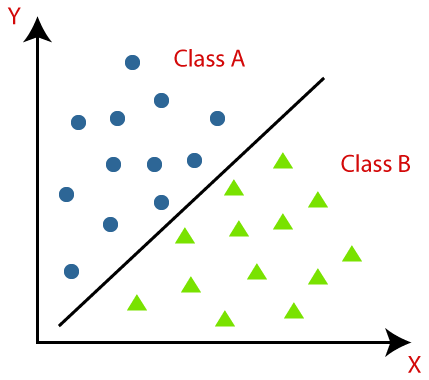
\includegraphics[height=.8\textheight]{classification-algorithm-in-machine-learning}
\end{frame}

\begin{frame}
  \frametitle{Области применения классификации в NLP}
  \begin{itemize}
  \item Документ целиком:
    \begin{itemize}
    \item  Определение языка текста
    \item Определение тематики текста (из набора известных тем)
    \item Sentiment classification (определение
      положительных/отрицательных отзывов)
    \item Определение автора текста (из списка кандидатов)
    \end{itemize}
  \item Отдельный токен (слово):
    \begin{itemize}
    \item Разделение текста на предложения (классификация точек)
    \item Определение части речи (part-of-speech tagging)
    \item Снятие омонимии (выбор значения слова)
    \item Извлечение именованных сущностей (Named entity recognition)
    \item Извлечение отношений (Relations extraction)
    \end{itemize}
  \end{itemize}
\end{frame}

\begin{frame}
  \frametitle{Задача машинного обучения}
  
Задача: \structure{научиться предсказывать трудно формализуемые, но
важные для человека свойства объекта (текста)}. 

  \begin{itemize}
  \item[target] Определить набор интересующих нас меток
  \item[features] Представить объект в виде набора свойств
  \item[model] На основании статистики распределения свойств в
    текстах построить модель, предсказывающую метки новых объектов
    (которых модель еще не видела).
    \pause
  \item \alert{PROFIT!}
  \end{itemize}
\end{frame}

\begin{frame}
  \frametitle{Классификация новых объектов}
  \centering
  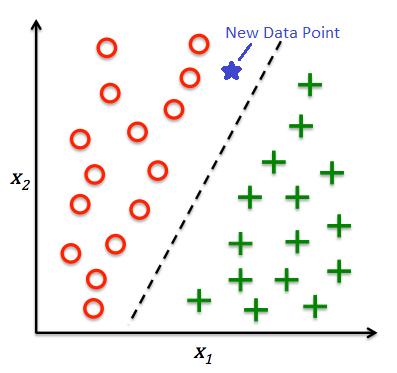
\includegraphics[height=.8\textheight]{new-data-point}
\end{frame}

\begin{frame}
  \frametitle{Разновидности машинного обучения}  
  \begin{description}
  \item[supervised] Обучение с учителем. 

    Модель учится предсказывать, опираясь на образцы меток,
    поставленных человеком.

  \item[unsupervised] Обучение без учителя. 

    Модель учится предсказывать на основании общих предположений о
    распределении свойств в текстах, без подготовленных человеком
    размеченных образцов.

  \item[semi-supervised] Обучение с использованием внешних знаний.
    
    Модель опирается на \alert{небольшое} количество размеченных
    человеком образцов и активное использование знаний о
    предметной области: словари понятий, распределения свойств и т.п.
  \end{description}
\end{frame}

\begin{frame}
  \frametitle{Терминология}
  \begin{description}
  \item[Обучающая выборка / training set]

    Набор объектов с выставленными человеком «правильными» метками, на
    основании которых строится («обучается») модель.

  \item[Тестовая выборка / test set]

    Набор объектов с выставленными человеком «правильными» метками, с
    помощью которых можно проверить, совпадают ли предложенные моделью
    метки с правильными.
    
  \end{description}
\end{frame}

\section{Проклятие размерности}

\begin{frame}[fragile]
  \frametitle{Sparse data problem}
\begin{verbatim}
    Terms
Docs выгребать выгребной выгружать выгрузка выгрызать
   1         0         0         0        0         0
   2         0         0         0        0         0
   3         0         0         0        0         0
   4         0         0         0        0         0
   5         0         0         0        0         0
\end{verbatim}
\end{frame}

\begin{frame}[fragile]
  \frametitle{Проклятие размерности}
  \framesubtitle{Curse of dimensionality}
\begin{verbatim}
A document-term matrix (1530 documents, 13322 terms)

Non-/sparse entries: 68859/20313801
Sparsity           : 100%
Maximal term length: 66 
Weighting          : term frequency (tf)
\end{verbatim}
\end{frame}

\begin{frame}
  \frametitle{Hughes phenomenon}
  \centering
  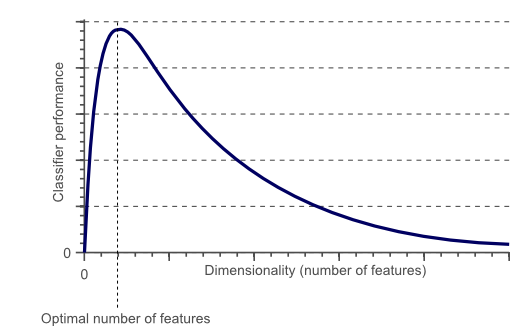
\includegraphics[width=.9\textwidth]{dimensionality_vs_performance}
\end{frame}

\begin{frame}
  \frametitle{Проклятие размерности на кошках}
  \centering
  \includegraphics<1>[width=.6\textwidth]{1Dproblem}
  \includegraphics<2>[width=.6\textwidth]{2Dproblem}
  \includegraphics<3>[width=.6\textwidth]{3Dproblem}
  \includegraphics<4>[width=.6\textwidth]{3Dproblem_separated}
\end{frame}

\begin{frame}
  \frametitle{Переобучение}
  \centering
  \includegraphics<1>[width=.6\textwidth]{overfitting}  
  \includegraphics<2>[width=.6\textwidth]{no_overfitting}  
\end{frame}


\section{Снижение размерности}

\begin{frame}
  \frametitle{Снижение размерности}
  \begin{itemize}
  \item Матрица терминов-документов очень большая и редкая
  \item Близкие по смыслу слова не обязательно встречаются в одних и
    тех же документах:
    \begin{itemize}
    \item синонимия
    \item полисемия
    \item шум
    \end{itemize}
    \pause
  \item Нужно сократить размерность матрицы (сделать меньше столбцов).
  \end{itemize}
\end{frame}

\begin{frame}
  \frametitle{Стоп-слова}
Простейший способ уменьшить число столбцов — просто \alert{удалить
  лишние слова}:

  \begin{itemize}
  \item Статический список:

без
более
бы
был
была
были
было
быть
в
вам
вас
весь
во
вот
все
всего
всех
вы
где
да
даже
для ...

  \item Динамический список:

    \begin{itemize}
    \item Слишком частотные (N самых частотных)
    \item Слишком редкие (порог: не менее чем в F документов)
    \item Слишком короткие (меньше M букв)
    \end{itemize}
  \end{itemize}
\end{frame}


\section{Оценка качества классификации}


\begin{frame}
  \frametitle{Accuracy}
  \begin{equation}
    \label{eq:a}
    Accuracy = \frac{P}{N}
  \end{equation}
  \begin{itemize}
  \item[$P$] количество документов, где классификатор принял
    правильное решение
  \item[$N$] размер обучающей выборки
  \end{itemize}
\end{frame}


\begin{frame}
  \frametitle{Таблица сопряженности}
  \framesubtitle{Contingency table}

  Таблица верных и неверных решений по документам данного класса:

  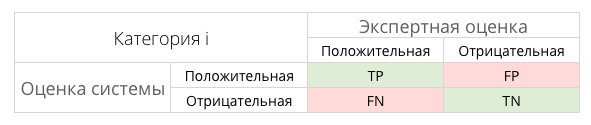
\includegraphics[width=\textwidth]{contingency-table}

  \begin{itemize}
  \item[TP] правильно отнесла к классу
  \item[TN] правильно не включила в класс
  \item[FP] ошибочно отнесла к классу
  \item[FN] ошибочно не включила в класс
  \end{itemize}
\end{frame}

\begin{frame}
  \frametitle{Точность и полнота}
  \begin{equation}
    \label{eq:p}
    Precision=\frac{TP}{TP + FP}
  \end{equation}
  \begin{equation}
    \label{eq:r}
    Recall=\frac{TP}{TP + FN}
  \end{equation}
\end{frame}


\begin{frame}
  \frametitle{Матрица неточностей}
  \framesubtitle{Confusion matrix}
  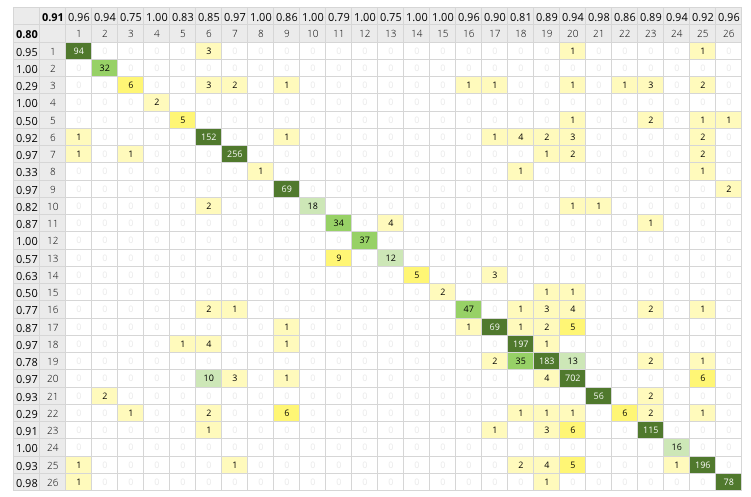
\includegraphics[height=.8\textheight]{confusion-matrix}
\end{frame}


\begin{frame}
  \frametitle{F-мера}
  \begin{equation}
    F_{\alpha} = \frac{(1+\alpha)PR}{\alpha P + R}
  \end{equation}

  \begin{equation}
    F_{1} = \frac{2PR}{P + R}
  \end{equation}  
\end{frame}


\begin{frame}
  \frametitle{Kappa}
  \begin{columns}
    \column{.5\textwidth}
    \begin{equation}
      \kappa = \frac{P_{\mathrm{observed}}-P_{\mathrm{expected}}}{1-P_{\mathrm{expected}}}
    \end{equation}
    \column{.5\textwidth}
    \begin{tabular}{r|ll|r}
     & коты  & собаки \\
      \hline
    коты & 20 & 5 & \alert{25}\\
    собаки & 10 & 15 & \alert{25} \\
    \hline
    & \alert{30} & \alert{20} & 
    \end{tabular}
  \end{columns}
  \only<2>{
    \begin{equation}
      P_{\mathrm{observed}} = (20 + 15)/50 = 0.7
    \end{equation}

    \begin{equation}
      P_{\mathrm{expected}} = ((25*30)/50 + (25*20)/50))/50 = (15 + 10)/50 = 0.5
    \end{equation}
 
    \begin{equation}
      \kappa = \frac{0.7 - 0.5}{1-0.5} = 0.4
    \end{equation}
}
\end{frame}


\end{document}
